\section{Durchführung}
\label{sec:Durchführung}
Die Bestandteile und der grundlegende Aufbau des Versuchs ist in Abbildung \ref{fig:grundlegenderAufbau} zu sehen. Es sind Aluminiumzylinder mit Durchmessern von 12,5, 50 und $\SI{75}{\milli\meter}$ vorhanden. Diese dienen dazu, den eindimensionalen Resonator nachzubilden. Dieser kann zwischen einem Mikrophon und einem Lautsprecher in einer Halterung aufgebaut werden. Für die Untersuchung des Kugelresonators als Analogie zum Wasserstoffatom stehen zwei Halbkugeln zur Verfügung. In einer der beiden befindet sich ein Mikrophon und in der anderen der Lautsprecher.\\

\begin{figure}
  \centering
  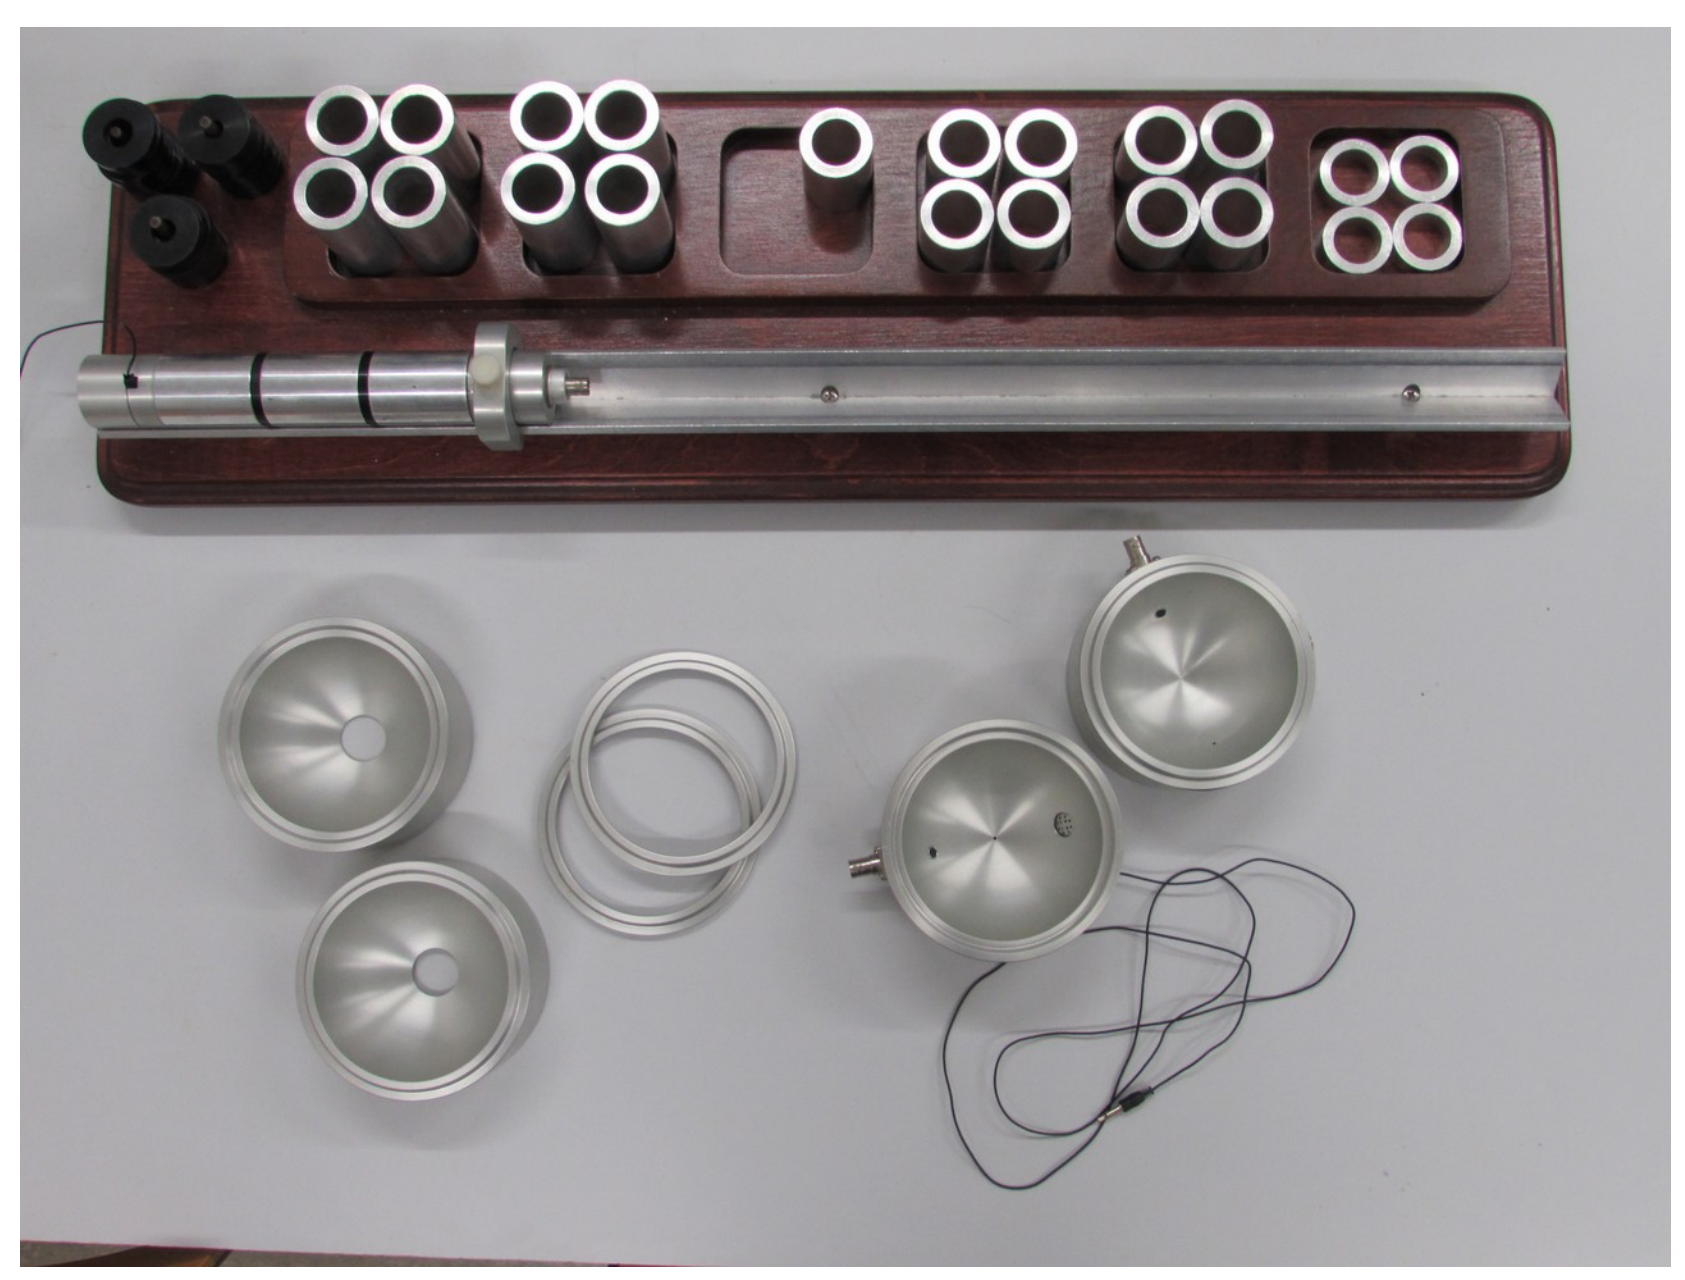
\includegraphics[width=\textwidth]{data/aufbau.png}
  \caption{Prinzipielle Bestandteile des Versuchs: Zylinder, Halterung und Halbkugelschalen \cite{Versuchsanleitung}.}
  \label{fig:grundlegenderAufbau}
\end{figure}

SKALA???????????\\
Eine mögliche Schaltung des Versuchs ist in \ref{fig:schaltung} schematisch dargestellt. Konkret wird dabei das Signal des Mikrophons am Oszilloskop untersucht. Inbesondere die Bestandteile des Steuergeräts sind dort sichtbar
Dieses verfügt über einen Eingang für das Mikrophon, dessen Signal einstellbar abgeschwächt werden und dann ausgegeben werden kann. Ein Frequenz-zu-Spannungs-Konverter ist vorhanden, sodass das Frequenzspektrum mit einem Oszilloskop oder mit einem Computer aufgenommen werden kann. Die Datenaufnahme am Computer geschieht mit dem Programm SpectrumSLC. Die Funktionalität umfasst die Aufnahme des Frequenzspektrums mit Einstellung der Schrittweite, Integrationszeit und Frequenzbereich. Ein Sinusgenerator dient zur Anregung der Resonanzen.\\

\begin{figure}
  \centering
  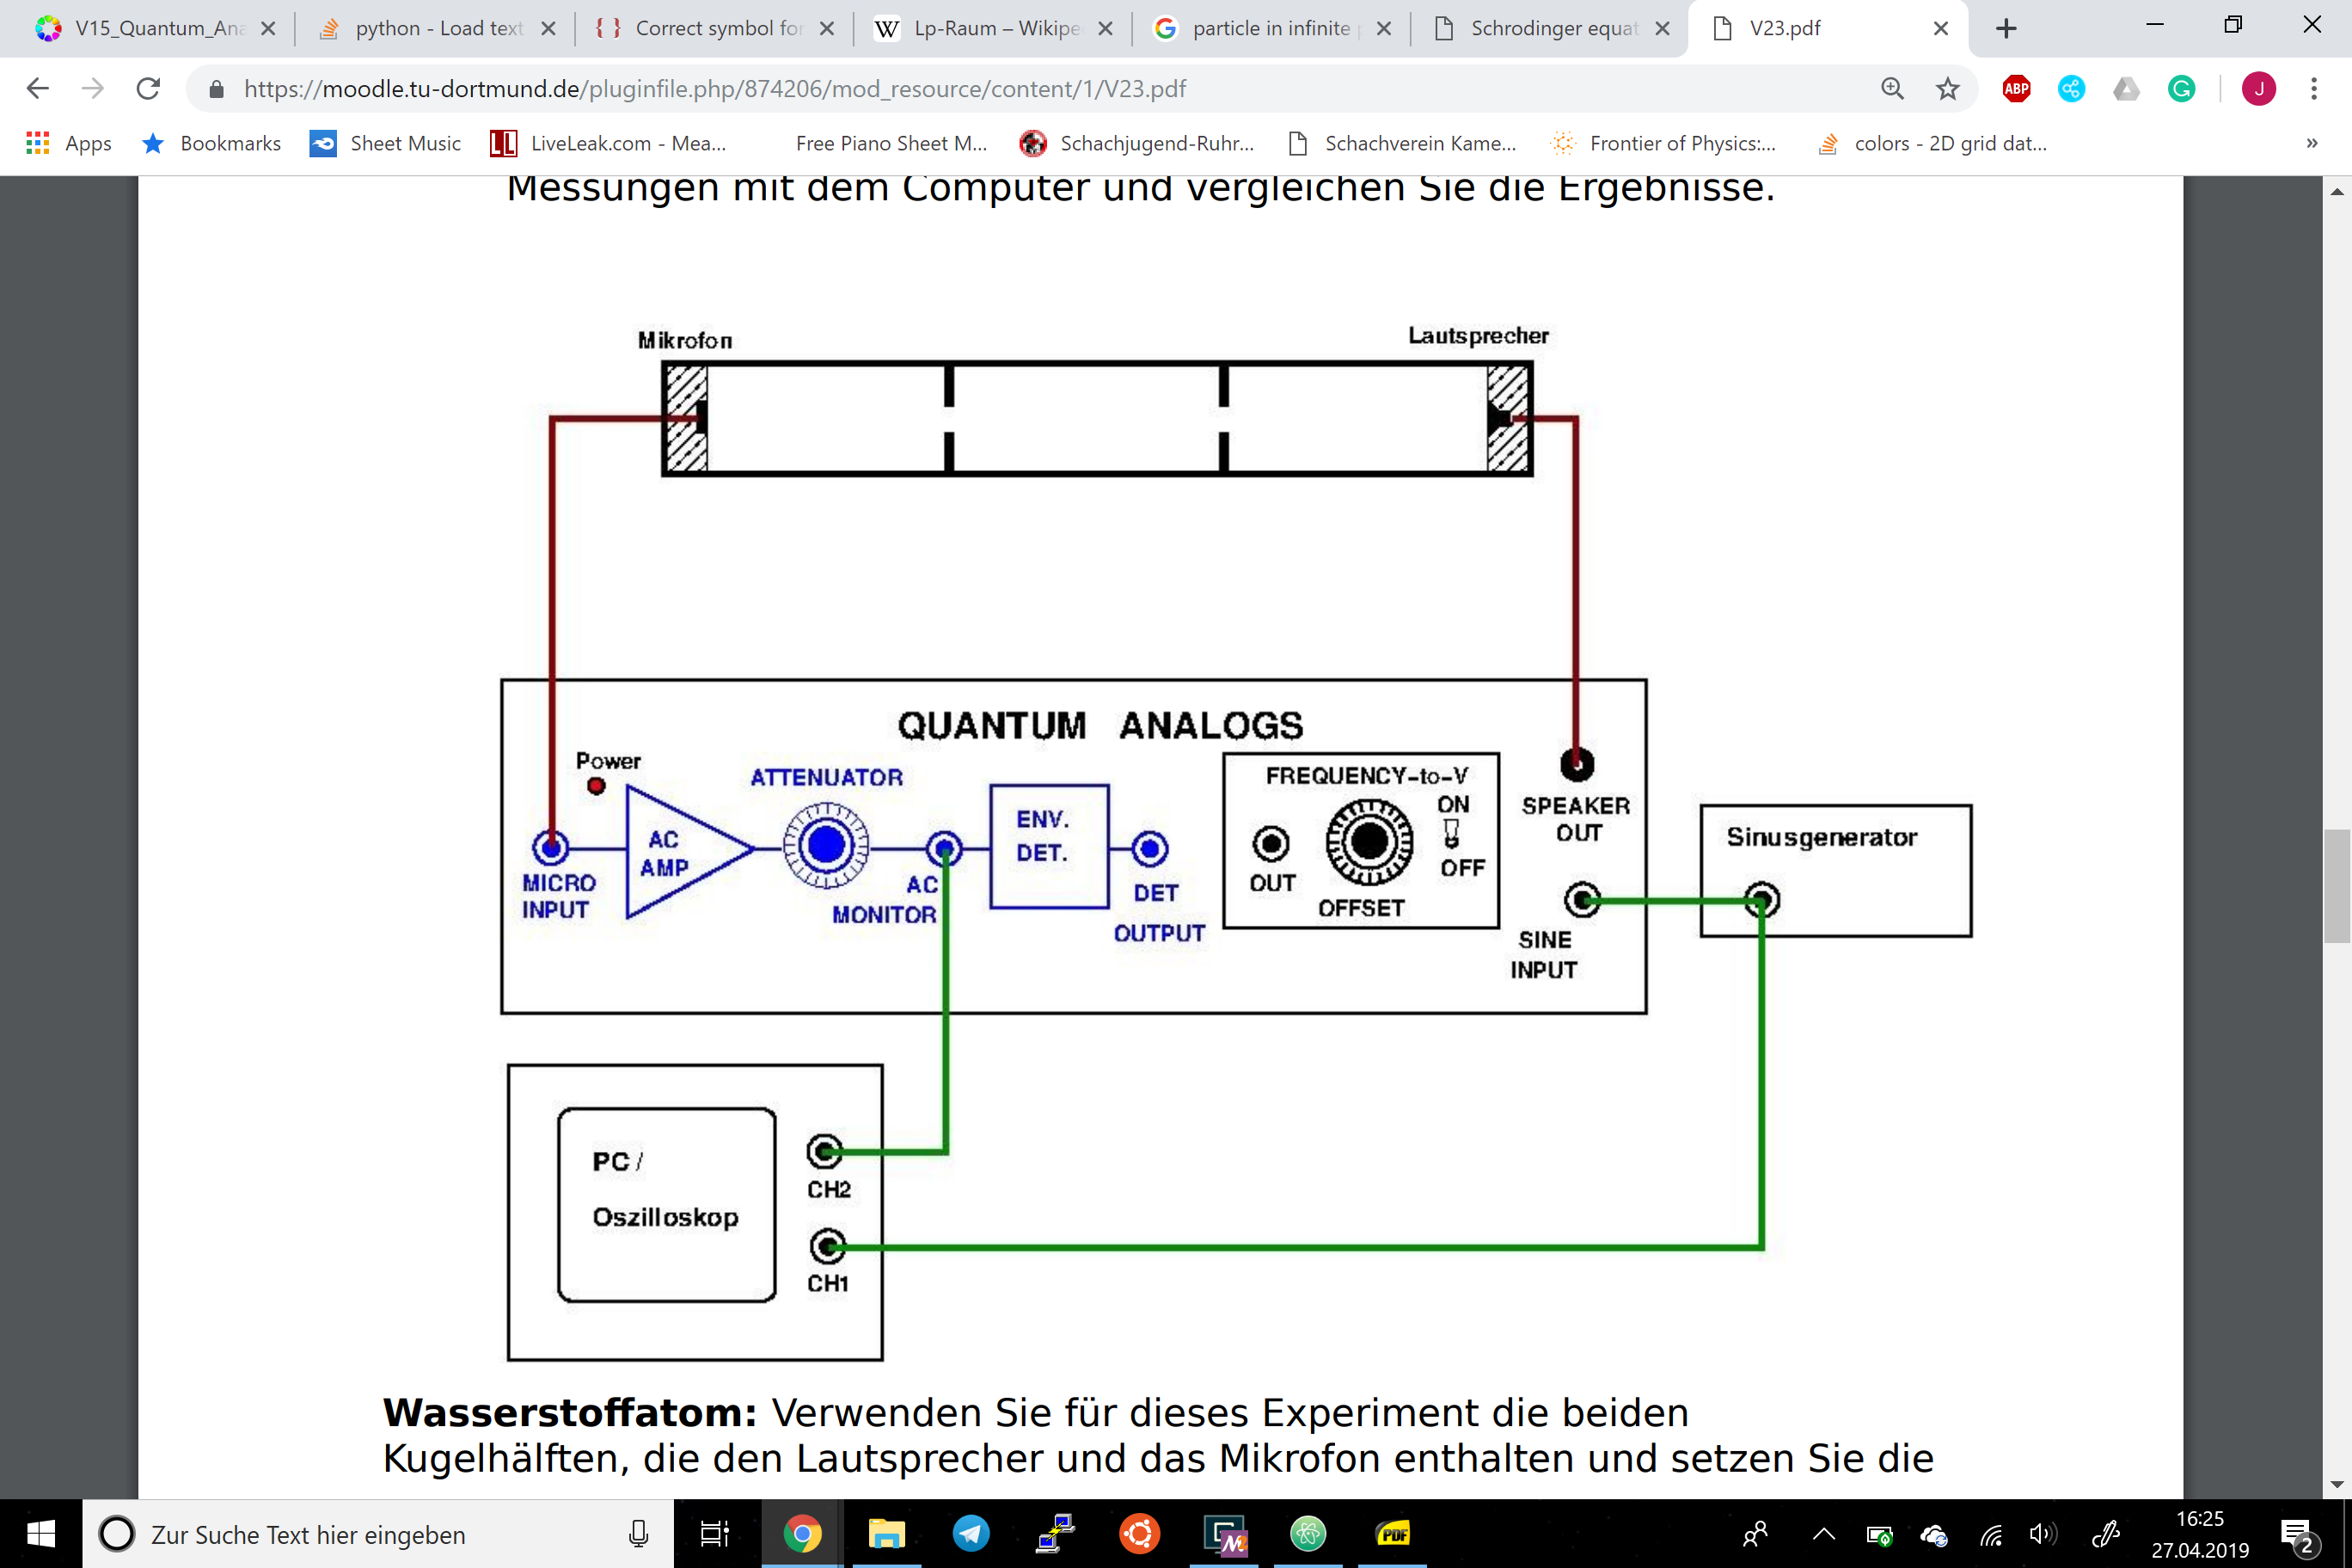
\includegraphics[width=\textwidth]{data/schaltung.png}
  \caption{Schematisches Schaltbild des Versuchs \cite{Versuchsanleitung}.}
  \label{fig:schaltung}
\end{figure}

\subsection{Durchführung vorbereitender Experimente}
\label{subsec:durchfuehrungVorbereitender}
Um sich mit dem Aufbau und dem Messprinzip vertraut zu machen, werden zwei Teilexperimente durchgeführt.\\
Im ersten Teilexperiment wird gemäß \ref{fig:schaltung} aufgebaut und die Signale am Oszilloskop untersucht. Ein Kanal des Oszilloskops stellt die Lautsprecherspannung und der andere die Mikrophonspannung dar. Der nun beschriebene Ablauf wird für 1,2,3,...,12 Zylinder wiederholt. Die Generatorfrequenz wird auf $\SI{6.75}{\kilo\hertz}$ geregelt. Dann wird sie erhöht, bis eine Resonanz am Oszilloskop ersichtlich ist. Dies ist genau dann der Fall, wenn die Amplitude im Vergleich zur Umgebung der Resonanzfrequenz maximal ist. Diese Frequenz wird gemeinsam mit der Amplitude UND WAS SONST NOCH SO? aufgezeichnet.\\\\
Das Ziel des zweiten Teilexperiments ist die Aufnahme des Frequenzspektrums für 1,2,3,...,12 Zylinder. Dabei sind die Ergebnisse der Aufnahme mit dem 2-Kanal-Oszilloskop und dem Computer zu vergleichen. Um mit dem Oszilloskop das Frequenzspektrum aufzunehmen, wird der xy-Modus gewählt. Der Frequenz-zu-Spannungs-Konverter wird auf den x-Eingang gelegt, auf die y-Achse wird die Amplitude der Resonanzen gelegt.
Der Sinusgenerator wird in seinen Sweep-Modus gestellt, das bedeutet, dass er einen manuell eingestellten Frequenzbereich in einer einestellbaren Zeit durchläuft. Das führt dazu, dass die aktuelle Amplitude der Schwingung über das Oszilloskop als Strich durchläuft. Resonanzfrequenzen drücken sich dann in einem stark vergrößerten Strich auf dem Oszilloskop aus. Da durch den Konverter ein Volt einem Kilohertz entspricht, ist bei Kenntnis der Anfangsfrequenz die Bestimmung der Lage der Resonanzfrequenzen möglich.\\
Der Aufnahme des Spektrums mit dem Computer geht der Anschluss der Lautsprecher- und Mikrophonausgänge am Experiment in die Eingänge des Computers voran. Danach wird die Messreihe aufgenommen. Die Daten liegen dann elektronisch als Messreihe Amplitude in willkürlicher Einheit und Frequnz vor.

\subsection{Der Kugelresonator}
Die beiden Kugelhälften werden aufeinander gesetzt. Zunächst stehen sich Lautsprecher und Mikrophon genau gegenüber, was $\alpha=180°$ entspricht. Die Durchführung dieses Teilversuchs besteht aus 5 Teilen.
\begin{itemize}
  \item Wieder wird mit dem Oszilloskop im xy-Modus ein Frequenzspektrum aufgenommen. Amplitude, Frequenz und Phasenverschiebung der Resonanzen werden aufgenommen. Der Messbereich ist 100 bis $\SI{10}{\kilo\hertz}$.
  \item Mit dem Computer wird für den selben Bereich ein Frequenzspektrum angefertigt.
  \item Ein Bereich, der drei Resonanzfrequenzen enthält, wird ausgewählt. Dieser Bereich wird für $\alpha$-Winkel von 0,10,20,... bis 180° vermessen.
  %\item Der $\SI{3}{\milli\meter}$ große Zwischenring wird zwischen die beiden Halbkugeln gesetzt
\end{itemize}
